% Diese Zeile bitte -nicht- aendern.
\documentclass[course=erap]{aspdoc}

%%%%%%%%%%%%%%%%%%%%%%%%%%%%%%%%%
%% TODO: Ersetzen Sie in den folgenden Zeilen die entsprechenden -Texte-
%% mit den richtigen Werten.
\newcommand{\theGroup}{208} % Beispiel: 42
\newcommand{\theNumber}{A405} % Beispiel: A123
\author{Uros Maletic \and Amir Taghizadegan \and Lukas Weng}
\date{Sommersemester 2020} % Beispiel: Wintersemester 2019/20
%%%%%%%%%%%%%%%%%%%%%%%%%%%%%%%%%

% Diese Zeile bitte -nicht- aendern.
\title{Gruppe \theGroup{} -- Abgabe zu Aufgabe \theNumber}

\usepackage{pgfplots}
\usepackage{pgfplotstable}

\begin{document}
\maketitle

\section{Einleitung}

Die Datenkompression ist ein Teilgebiet der Kodierungstheorie und beschäftigt sich damit, wie man den Speicherbedarf von Datenmengen auf ein Minimum reduzieren kann.\cite{codierungstheorieVT}
Man unterscheidet zwischen verlustfreier und verlustbehafteter Datenkompression. Bei der verlustfreien Kompression enthalten die verdichteten Daten den ursprünglichen Inhalt noch vollständig und es kann durch Dekodierung der originale Code wiederhergestellt werden. Diese Kompressionsart wird unter anderem bei Text- oder Programmdateien angewendet.
Bei der verlustbehafteten Kompression bleibt der Inhalt zwar in den Grundzügen erkennbar, es können aber Informationen verloren gehen, um den Speicherbedarf noch weiter zu optimieren. Man muss somit die dargestellte Informationsmenge gegenüber dem Speicherbedarf abwägen. Beispielsweise bei Bild- oder Audiodateien ist diese Kompressionsart sinnvoll.\cite{grundkursCodierungSpringer}

Im Folgenden wird eine Implementierung der Huffmankodierung vorgestellt, welche in Assembler erstellt wurde. Die Huffmankodierung ist ein verlustfreies Kompressionsverfahren, bei dem präfix-freier Code generiert wird. Präfix-frei bedeutet, dass kein Codewort Anfang eines anderen Codeworts ist und dadurch keine Trennzeichen bei der Speicherung des neu kodierten Worts nötig sind.
Wie die meisten Kompressionsverfahren dieser Art folgt die Huffmankodierung dem Grundprinzip, dass häufig auftretende Symbole durch kurze Codewörter und selten vorkommende Symbole durch lange Codewörter beschrieben werden. Die Codewörter haben somit unterschiedliche Längen, können aber, da die Menge alle Codewörter präfix-frei ist, direkt und eindeutig identifiziert werden.

Die Kodierung nach dem Huffmanalgorithmus teilt sich in drei Schritte: Zuerst wird eine Häufigkeitsanalyse auf dem Eingabewort durchgeführt, die die absoluten Häufigkeiten aller Symbole bestimmt und daraus eine sortierte Häufigkeitstabelle erstellt. Um aus der Häufigkeitstabelle die Codewörter mit optimalen Längen zu generieren, wird im zweiten Schritt ein sogenannter Codebaum erstellt, der den Symbolen die Codewörter nach dem zuvor beschriebenen Prinzip der Häufigkeit zuordnet und die Kodierungen in eine Tabelle schreibt. Diese Tabelle wird Wörterbuch genannt. Zuletzt wird das Eingabewort in die neue Kodierung übersetzt.\cite{codierungUndKryptologieSpringer}

Eine Besonderheit des Huffmanverfahrens ist, dass der generierte Code optimal ist, das heißt die mittlere Codewortlänge kann nicht weiter reduziert werden. Die mittlere Codewortlänge gibt die Summe der nach den Auftrittswahrscheinlichkeiten gewichteten Codewortlängen an und entspricht damit dem Erwartungswert der Codewortlänge.\cite{codierungstheorieVT}\\

\section{Lösungsansatz}

Dieser Abschnitt beschäftigt sich mit der genauen Funktionsweise und Umsetzung des Huffmanalgorithmus und unterteilt sich in die drei zuvor beschriebenen Schritte.\\Die implementierte Funktion hat folgende Signatur:\\\textit{int huffman\_encode(char *data, char *result, unsigned int result\_size)}

Im data-Array werden die zu kodierenden Daten übergeben, deren Ende durch ein Nullbyte markiert ist. In das result-Array werden von der Funktion zuerst das Wörterbuch, dann ein Trennbyte und zuletzt die neu kodierten Daten geschrieben. Die Größe des result-Arrays wird als weiterer Parameter übergeben. Die Rückgabe der Funktion ist -1, falls ein Fehler aufgetreten ist und sonst die Anzahl der benötigten Bytes für Wörterbuch, Trennbyte und Kodierung. Es können nur Zeichen aus der klassischen 7-Bit-ASCII-Variante kodiert werden.\\

\subsection{Häufigkeitsanalyse}

Die Häufigkeitsanalyse erstellt eine Tabelle, die alle im Eingabewort vorkommenden Zeichen mit der zugehörigen Häufigkeit beinhaltet. Zum Abspeichern der Häufigkeitstabelle wird das result-Array verwendet, da diese nur als Zwischenergebnis für die Erstellung des Codebaums benötigt wird. Die Häufigkeitstabelle wird abwechselnd mit jeweils zwei Bytes für ein Zeichen und dann zwei weiteren Bytes für dessen Häufigkeit abgespeichert, wobei die Tabelle nach den Häufigkeiten absteigend sortiert ist. Im kleinsten Fall, das heißt bei einem Eingabewort, das nur ein Zeichen verwendet, kann mit dieser Variante eine Eingabe mit (2\textsuperscript{16} - 1) = 65535 Zeichen verarbeitet werden. Im größten Fall, das heißt bei einem Eingabewort in dem alle 126 Zeichen mit maximaler Häufigkeit vorkommen, kann man mit der Implementierung ein Eingabewort der Länge 126 x (2\textsuperscript{16} - 1) = 8.257.410 analysiert werden. Sollte die Häufigkeit eines Zeichens zu groß für die Speicherung in zwei Bytes sein, wird dies erkannt und führt zum Abbruch des Programms. Der Algorithmus zur Häufigkeitsanalyse wird hier an der Beispieleingabe \textit{AADZDAADDZAAAADAZZD} vorgestellt.

In einer äußeren Schleife wird über die zu verarbeitenden Daten iteriert, das heißt es wird im ersten Schritt das Zeichen 0 aus dem data-Array geladen. Anschließend iteriert man in einer inneren Schleife über das data-Array und zählt, wie häufig das aktuelle Zeichen ‚A‘ vorkommt. Für den Zählvorgang wird zuerst abgefragt wie viele Zeichen zu überprüfen sind. Dies hat zwar zur Folge, dass zu Beginn der Häufigkeitsanalyse ermitteltet werden muss, wie groß das data-Array ist, es ermöglicht aber SIMD-Operationen einzusetzen.

Falls mindestens 16 Zeichen verglichen werden müssen, werden SIMD-Operationen verwendet. Hierzu wird zuerst eine Maske erstellt, die in einem xmm-Register 16mal das zu vergleichende Zeichen enthält. Dann werden die ersten 16 Zeichen aus dem data-Array mit der Maske verglichen. Der Vergleich generiert eine neue Maske, welche -1 an den Bytes enthält, die beim Vergleich übereingestimmt haben und sonst 0.

Die Performanz wird durch das geforderte 16-Byte-Alignment der SIMD-Operationen etwas eingeschränkt, da immer nur ab Adressen, die ein Vielfaches von 16 sind, verglichen werden kann. Das Setzen des Zählers auf eine Adresse n, die ein Vielfaches von 16 ist, das heißt das Berechnen von  n – (n\%16) kann effizient mit einer and-Operation ausgeführt werden, welche die unteren vier Bits auf Null setzt. Der Einsatz von SIMD-Operationen sollte dennoch sinnvoll sein, da insbesondere wegen der Größe von jeweils nur einem Byte der zu vergleichenden Daten in Durchschnitt eine gute Anzahl parallel ausgeführter Vergleiche erzielt wird. Die Frage, ob die Performanz durch SIMD-Operationen bei diesem Algorithmus tatsächlich gesteigert werden konnte, wird in Abschnitt \ref{performanzAnalyse} Performanzanalyse beantwortet.\\
\begin{figure}[h]
\begin{center}
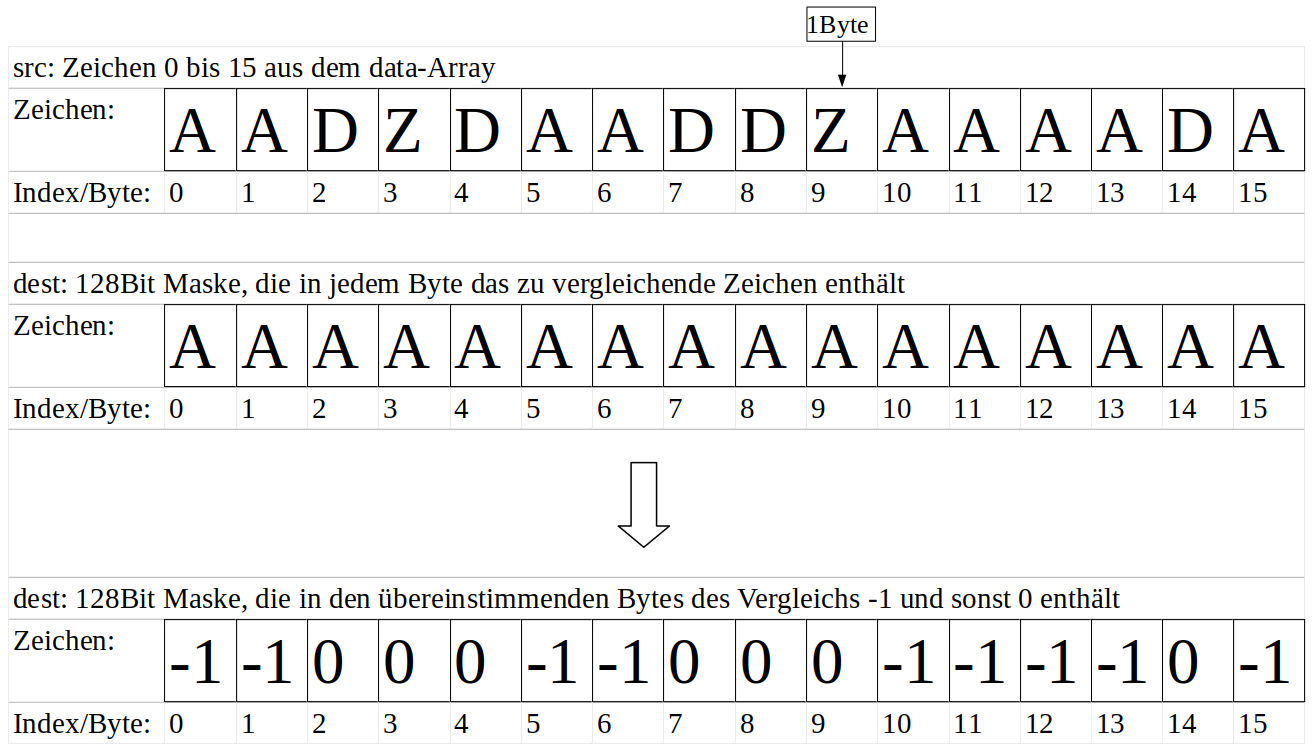
\includegraphics[scale=0.3]{resourcen/abb1.png}
\caption{Durchführung des ersten SIMD-Vergleichs}
\label{abb2}
\end{center}
\end{figure}
\\
Die aus dem Vergleich generierte Maske hat zwei Zwecke.\\
Zum ersten werden damit die Zeichen, die bereits gezählt wurden im data-Array auf -1 gesetzt werden. Dies hat zwar zur Folge, dass das später nochmals benötigte data-Array zu Beginn der Analyse gesichert werden muss, jedoch ist die Überprüfung ob ein Zeichen bearbeitet wurde zu Beginn der äußeren Schleife deutlich schneller möglich. Alternativ müsste bei der Auswahl des nächsten zu überprüfenden Zeichens jedes mal das result-Array oder ein anderer Zwischenspeicher durchlaufen werden, um abzufragen ob das Zeichen bereits dort eingetragen wurde. Der Performanzgewinn, insbesondere die deutlich geringere Anzahl an Speicherzugriffen, überwiegt damit gegenüber dem Aufwand beim Sichern.\\
\begin{figure}[h]
\begin{center}
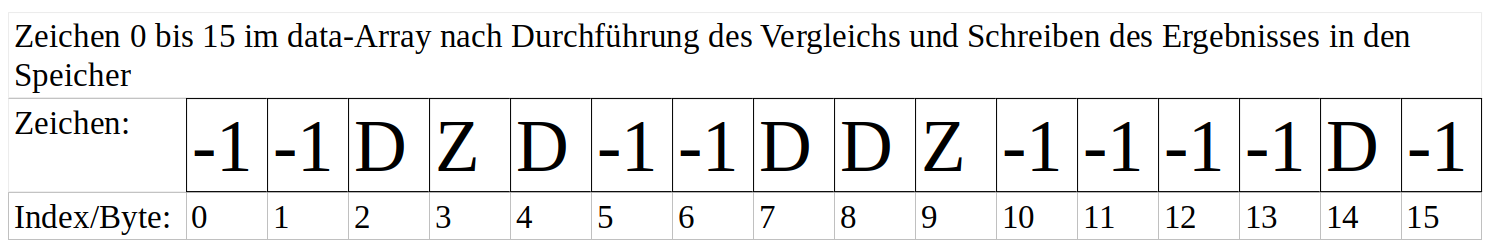
\includegraphics[scale=0.2633]{resourcen/abb2.png}
\caption{Zeichen 0 bis 15 im data-Array nach Rückschreiben der Ergebnisse der Vergleichs}
\label{abb3}
\end{center}
\end{figure}
\\
\\Zum zweiten kann mit der Maske die eigentliche Aufgabe des Zählens erledigt werden. Dafür werden alle Bytes, welche den Wert -1 haben durch eine and-Operation effizient auf 1 gesetzt. Anschließend werden alle Bytes der Maske aufsummiert und das Zwischenergebnis zum Häufigkeitszähler des aktuellen Zeichens addiert.


Die verbleibenden zu vergleichenden Zeichen werden mit SISD-Operationen bearbeitet. Auch hier werden gezählte Zeichen im data-Array auf -1 gesetzt. Nachdem das gesamte data-Array mit dem aktuellen Zeichen verglichen wurde, wird das Zeichen und danach die ermittelte Häufigkeit mit jeweils zwei Bytes in das result-Array geschrieben.


In der nächsten Iteration der äußeren Schleife wird beim Auslesen des Zeichens 1, welches ein ‚A‘ war, durch die -1 direkt erkannt, dass es schon bearbeitet wurde und es kann sofort mit dem Bearbeiten des Zeichens 2: ‚D‘ begonnen werden. Obwohl das ‚D‘ eigentlich mit den Zeichen 3 bis 18  verglichen werden können, muss es aufgrund des 16-Byte-Aligments mit den Zeichen 0 bis 15 verglichen werden.


Nachdem die Häufigkeiten aller Zeichen gezählt wurden, wird das noch unsortierte result-Array mithilfe des Quicksort-Algorithmus nach den Häufigkeiten absteigend sortiert und kann zur Erstellung des Codebaums verwendet werden. Zeichen mit gleichen Häufigkeiten haben keine innere Ordnung, da dies für den Huffmanalgorithmus nicht relevant ist. Nachfolgende Abbildung zeigt das Ergebnis der Häufigkeitsanalyse für das Beispiel.\\
\begin{table}[h]
\centering
\begin{tabular}{ | c | c | }
 \hline
 Symbol & Häufigkeit \\
 \hline
 A & 9 \\
 \hline
 D & 6 \\
 \hline
 Z & 4 \\
 \hline
\end{tabular}
\caption{Ergebnis der Häufigkeitsanalyse für das Beispiel}
\end{table}
\\
Neben dem Fehler, dass mindestens ein Zeichen zu häufig vorkommt, wird auf den Fall, dass ein Zeichen im Eingabewort nicht von der 7-Bit-ASCII-Variante kodiert wird und den Fall, das das result-Array zu klein ist, reagiert. Die Fehlererkennung wird erst zum Zeitpunkt des möglichen Auftretens, beispielsweise direkt bevor über die Grenzen des result-Arrays geschrieben würde, gemacht das heißt es wurde bewusst von einer Überprüfung der Eingabe zu Beginn des Programms abgesehen, wodurch Fehler früher abgefangen werden könnten. Zwar dauert es damit besonders bei großen Eingabedaten länger, bis eventuelle Fehler erkannt werden, dafür ist die Performanz des Programms bei korrekter Verwendung höher.\\
\label{analyse}

\subsection{Erstellung des Wörterbuchs}
\label{wörterbuch}
Der wichtigste Teil bei der Erstellung des Wörterbuchs ist der korrekte Aufbau des Huffmanbaums.\cite{huffmanArticle} Die Knoten der Bäume werden in C normalerweise als selbst definierte zusammengesetzte Datentypen oder auch Strukturtypen deklariert. Diese besitzen immer eine Referenz auf die jeweiligen Kinder. \cite{cAlsErsteProgrammiersprache} Da ein Huffmanbaum ein unvollständiger Binärbaum ist, enthält dieser immer zwei Zeiger auf den linken und rechten Teilbaum. Um diese Datenstruktur zu realisieren, muss für jeden Knoten Speicherplatz reserviert werden. Dies wird mit dem System Call 0x9 - mmap realisiert. Es werden pro Knoten, um das acht Byte Alignment zu erhalten, 24 Bytes alloziert. Von den ersten acht Bytes werden nur die ersten vier Bytes belegt. Die erste Hälfte der vier Bytes dient der Speicherung des Buchstabens und die Zweite der Speicherung der Häufigkeit des gleichen. Die zweiten acht Bytes sichern den Zeiger auf den linken Knoten und die Letzten enthalten den Zeiger auf den rechten Teilbaum.


Am Anfang wird für jeden Charakter und seine Häufigkeit ein Knoten erstellt und seine Werte initialisiert. Die Pointer auf diese Knoten werden aufsteigend sortiert nach ihrer Häufigkeit in einen Haufen eingefügt. Der Speicher für den Heap wird auch mittels System Call 0x9 alloziert. Die Größe dafür beträgt der Anzahl an Knoten multipliziert mit acht (wegen der Größe der Pointer) sowie noch weitere acht Bytes für Informationen über das Array. Die erste Hälfte der acht Bytes wird verwendet, um abzuspeichern, wie viele Bytes alloziert wurden und die zweite Hälfte beinhaltet die Anzahl an Teilbäumen im Datenfeld. Diese \enquote{Informationsbytes} befinden sich am Anfang des Arrays.\\\\
Nach dem Einfügen fängt die Generierung des Baums an. Zuvor wird noch auf die Referenz, welche auf den Haufen zeigt, acht addiert damit diese auf den Knoten mit der kleinsten Häufigkeit zeigt. Dieser und der nächstkleinere Knoten werden \enquote{zusammengeführt}\cite{codierungUndKryptologieSpringer} d. h. die Häufigkeiten dieser zwei Knoten werden summiert und ein neuer Knoten mit der Summe erzeugt, als Zeichen wird das Dummy-Zeichen 0x1 benutzt. Diese Zahl repräsentiert kein darstellbares Symbol aus der ASCII-Kodierung und dient lediglich der Bezeichnung der \enquote{zusammengeführten}\cite{codierungUndKryptologieSpringer} Knoten. Der Zeiger auf das linke Kind wird mit dem Pointer auf den kleineren der zwei Knoten belegt und der rechte Zeiger dementsprechend mit dem Größeren. Die Anzahl an Elementen wird um eins reduziert und der neue Knoten wird zunächst an der Stelle des Knotens mit der zweitkleinsten Häufigkeit eingefügt. Danach wird der neue Teilbaum durch das Vertauschen der Teilbäume an die richtige Stelle gebracht, sodass wieder alle Knoten aufsteigend nach der Häufigkeit sortiert sind. Dies wird solange wiederholt bis nur noch ein Baum übrig ist.  Dies ist der Codebaum, welcher traversiert wird um das Wörterbuch zu erstellen. Falls die Höhe des Baums mehr als acht beträgt, wird hier abgebrochen und -1 zurückgegeben.\\\\
Um die Wirksamkeit der Kodierung beizubehalten, muss das Wörterbuch auch dementsprechend klein sein.\cite{grundkursCodierungSpringer} Das wurde bei dieser Implementierung dadurch erreicht, dass nur die 7-Bit-ASCII-Zeichen kodiert werden. Jeder Eintrag im Wörterbuch beträgt zwei Bytes. Das zweite Byte speichert das Codewort und die niedrigen sieben Bits des ersten Bytes besitzen den Buchstaben der kodiert werden soll. Das oberste Bit wird benutzt um zu bestimmen, ob das Codewort mit einer Eins oder einer Null anfängt. Dadurch dass bei der Huffmankodierung die Codes unterschiedliche Längen haben, muss man genau wissen wie lang das Codewort ist. Diese Längenangabe müsste bei dem Extended-ASCII-Code durch ein zusätzliches Byte erfolgen. Ein Beispiel Eintrag sieht dann so aus: 01000001 11111110. Da das oberste Bit auf Null gesetzt wurde, fängt das Codewort mit einer Null an, weswegen alle Bits davor auf Eins gesetzt werden. Wäre das oberste Bit eine Eins so werden alle Bits davor auf Null gesetzt. Hierdurch lassen sich die Einträge im Wörterbuch durch zwei Bytes darstellen.


Die Traversierung erfolgt dann rekursiv. Zuerst wird das linke Kind der Wurzel durchgearbeitet. Hierbei muss man unterscheiden, dass die linke Kante eine Null zum Anfang des Codeworts hinzufügt. Wie schon erklärt, werden deswegen alle Bytes des Codeworts auf Eins gesetzt und um Eins nach links geshiftet. Das temporäre Codewort wird im Register cl abgesichert. Das Bit welches indiziert, womit das Codewort anfängt wird im Register cl gespeichert, in diesem Fall bleibt es leer. Vor dem rekursiven Aufruf der Methode wird noch das Register rdx auf den Stack draufgelegt, so bleibt das Codewort beim Aufruf auf das nächste Kind unverändert. Wenn ein Knoten erreicht wird, in dem ein anderes Symbol als das Dummy-Zeichen steht, wird das Symbol sowie das Codewort dieses Zeichens in das result-Feld kopiert und entsprechend das oberste Bit gesetzt oder nicht. Nach dem gleichen Prinzip wird auch das rechte Kind der Wurzel traversiert. Dieses Mal wird aber dl geleert und bei cl das oberste Bit auf Eins gesetzt. Am Ende der Traversierung wird noch ein Byte mit einer Eins gefüllt, dieses Byte teilt das Wörterbuch von der Kodierung im result-Array.\\

\begin{table}[h]
\centering
\begin{tabular}{ | c | c | c | }
\hline
 Buchstabe & Codewort & Im Speicher\\
\hline
 A & 1 & 01000001 11111110\\
\hline
 D & 01 & 11000100 00000011\\
\hline
 Z & 00 & 11011010 00000010\\
\hline
\end{tabular}
\caption{Wörterbuch für das Beispiel aus \ref{analyse}}
\end{table}
\subsection{Übersetzung}
Der letzte Schritt des Huffmanalgorithmus ist die Übersetzung des Eingabeworts in die neue Kodierung. Dieser unterteilt sich in fünf Hauptschritte, die für jedes Quellsymbol des Eingabeworts wiederholt werden: 
\begin{enumerate}
	\item Ein Quellsymbol aus dem Eingabewort wird gelesen.
	
	\item Das zugehörige Codewort wird aus dem zuvor erstellten und in result übergebenen Wörterbuchs ermittelt.
	
	\item Das Codewort wird angepasst und in ein 64 Bit Register kopiert.
	
	\item Die Kodierung wird in ein 64 Bit Puffer auf dem Stack gespeichert. 
	
	\item Falls der Puffer schon voll ist, wird er im result-Array an passender Stelle herausgeschrieben und anschließend geleert. Der Teil von dem letzten Codewort, der evtl. nicht mehr in den letzten Puffer kopiert werden konnte, wird in den neuen Puffer kopiert.
	
	 
\end{enumerate}
Die Realisierung dieser Schritte werden nun im Folgenden genauer erklärt und durch die Kodierung des Zeichens 'Z' (erstes Vorkommen) in der Beispieleingabe \\ \textit{AADZDAADDZAAAADAZZD} verdeutlicht: 

Zu Schritt 2: Um den Wörterbucheintrag, der zu dem aktuellen Quellsymbol passt, zu finden, wird das Wörterbuch durchlaufen. Dabei wird das obere Byte des Eintrags mit dem Quellsymbol verglichen. 
Wie bereits in \ref{wörterbuch} erwähnt, gibt das oberste Bit eines Wörterbucheintrags an, ob das Codewort mit einer 0 oder einer 1 anfängt. Die 7 Bits danach geben den Buchstaben an. Da ein Vergleich mit 7 Bits aufwändig ist, wird das oberste Bit des Quellsymbols entsprechend des obersten Bits des Wörterbucheintrags gesetzt. 
Anschließend werden die zwei Bytes, das heißt das modifizierte Quellsymbol und das obere Byte des Wörterbucheintrags verglichen. Wenn diese gleich sind, ist der richtige Eintrag gefunden worden und falls nicht, wird der Ablauf mit dem nächsten Wörterbucheintrag wiederholt.\\
\begin{table}[h]
	\centering
	\begin{tabular}{lllll}
		\cline{3-3}
		Quellsymbol& \multicolumn{1}{l|}{}& \multicolumn{1}{l|}{0\hspace{0.2cm}1011010} &&  \\ 
		\cline{3-3}&&&&\\ 
		\cline{3-4}
		Wörterbuch: & \multicolumn{1}{l|}{...} & \multicolumn{1}{l|}{1{$\underbrace{1011010}_{Buchstabe: Z}$}} & \multicolumn{1}{l|}{{$\underbrace{00000010}_{Codewort}$}} & ... \\ \cline{3-4}
		& & \multicolumn{1}{c}{||}&&
		\\ \cline{3-3}
		Quellsymbol modifiziert: & \multicolumn{1}{l|}{}& \multicolumn{1}{l|}{1\hspace{0.2cm}1011010} && \\ 
		\cline{3-3}
	\end{tabular}
\end{table}
\\
Zu Schritt 3: Nun nachdem der passende Wörterbuch Eintrag gefunden wurde, wird nicht das komplette Codewort in den Puffer geschrieben, sondern nur die komprimierte Form (Kodierung). Um das zu erreichen, wird zuerst herausgefunden wo die Kodierung, die variable Länge haben kann, im Codewort anfängt. Das oberste Bit im Wörterbucheintrag erweist sich hier als nützlich. Falls die Kodierung nämlich mit einer 0 anfängt, geht man im Codewort Bit für Bit weiter, bis man auf eine 0 stößt und wenn die Kodierung mit einer 1 anfängt umgekehrt. Anschließend werden die oberen Bits davor auf 0 gesetzt und das modifizierte Codewort in ein leeres 64 Bit Register kopiert. 

Zu Schritt 4: Bevor das modifizierte Codewort (64 Bit jetzt) mit dem 64 Bit Puffer addiert wird, sollte die Kodierung an die richtige Stelle (nächste freie Stelle im Puffer) gebracht werden. Im r8 Register steht der Index des ersten freien Bits vom Puffer. Falls der Puffer genug Platz für die neue Kodierung hat, wird die Kodierung durch ein Links Shift an die Stelle, die in r8 steht gebracht. Anschließend wird das modifizierte Codewort mit dem Puffer addiert und die neue Kodierung somit in den Puffer eingefügt. Der Rest vom Puffer wird dabei nicht verändert, da vor und nach der Kodierung nur Nullen stehen.\\
\begin{table}[h]
	\centering
	\begin{tabular}{lllll}
		\cline{2-2}
		\multicolumn{1}{l|}{Codewort in 64 Bit Register:}& \multicolumn{1}{l|}{0000000...00000\textbf{10}}                                  &&& \\ 
		\cline{2-2}
		&                                                                    &  &  & \\ 
		\cline{2-2}
		\multicolumn{1}{l|}{Codewort geshiftet:}& \multicolumn{1}{l|}{0000\textbf{10}0...0000000}                                 &  &  &  \\ 
		\cline{2-2}
		& \multicolumn{1}{c}{+}                                                                                              &&&  \\ \cline{2-2}
		\multicolumn{1}{l|}{Puffer:} & 
		\multicolumn{1}{l|}{
			\begin{tabular}[c]{@{}l@{}}0011000...0000000\\
				\hspace{0.77cm}↑\\ \hspace{0.5cm} r8 (erstes freies Bit)
		\end{tabular}} &  &  &  \\ \cline{2-2}& \multicolumn{1}{c}{=}                                                                                              &  &  &  \\ \cline{2-2}
		\multicolumn{1}{l|}{Puffer mit der neuen Kodierung:} & \multicolumn{1}{l|}{
			\begin{tabular}[c]{@{}l@{}}0011\textbf{10}0...0000000\\
				\hspace{1.15cm}↑\\ \hspace{0.5cm} r8 (erstes freies Bit)
		\end{tabular}} &  &  &  \\ \cline{2-2}
	\end{tabular}
\end{table}
\\
Nun kann es jedoch den Fall geben, dass der Puffer nicht genug Platz hat und das Codewort nach Rechts anstatt nach Links geshiftet werden muss. Das hat aber den Effekt, dass ein Teil der Kodierung nun abgeschnitten wird. Im nächsten Schritt wird dieser Teil jedoch in den neuen Puffer eingefügt.


Zu Schritt 5: Nach einigen Durchläufen wird der Puffer voll werden und muss deshalb in das result-Array geschrieben werden. Die neuen Kodierungen werden dabei nach dem 1-Byte-Splitter und nach den evtl. bereits zuvor eingefügten Kodierungen gespeichert. Anschließend wird der Puffer auf 0 gesetzt, der Teil der neuesten Kodierung, der nicht mehr gespeichert werden konnte darin eingefügt und durch ein Links-Shift an die erste/oberste Stelle gebracht.\\\\
Nach der Beendigung der obigen Schleife wird noch der letzte Puffer in das result-Array abgespeichert, falls er noch Daten enthält. Hier wird jedoch evtl. nicht der gesamte 8-Byte Puffer herausgeschrieben, sondern nur so viele Bytes, die verwendet wurden. Falls im letzten Puffer beispielsweise noch 34 Bits eingefügt wurden, werden zuerst vier Bytes herausgeschrieben und dann noch ein letztes Byte. Es fällt sofort auf, dass in diesem Fall die restlichen sechs Bits des letzten Bytes nicht mehr zu der Kodierung gehören. Damit dies auch bei der Dekodierung erkennbar ist, muss das Ende markiert werden. Das zweite Bit des Splitters gibt deshalb an, ob die Kodierung mit einer 1 oder einer 0 endet. Falls die Kodierung mit einer 0 endet, werden die Bits des letzten Bytes, die nicht mehr zu der Kodierung gehören, zusätzlich auf 1 gesetzt. Falls die Kodierung mit einer 1 endet sind diese Bits bereits 0.    

Außerdem sei noch erwähnenswert, dass jedes Mal nachdem die Länge der Kodierung eines Quellsymbols bekannt ist (nach Schritt 3), überprüft wird, ob noch im result-Array genug Platz vorhanden ist. Falls dies nicht der Fall ist, wird das Programm abgebrochen und es wird -1 zurückgegeben. Ansonsten wird die Länge des gesamten Codes in Bytes zurückgegeben.
Diese Länge wird später im Rahmenprogramm nützlich sein, um den verwendeten Teil des result-Arrays in die Ausgabedatei zu schreiben.


Zuletzt sollte noch gesagt werden, dass es auch möglich wäre jede Kodierung als Byte direkt nach Schritt 3 in das result-Array zu schreiben. Dies würde jedoch die Anzahl der Speicherzugriffe deutlich erhöhen, weshalb wir uns für ein 64 Bit Puffer entschieden haben. 




% TODO: Je nach Aufgabenstellung einen der Begriffe wählen
\section{Korrektheit}

Wird das Rahmenprogramm mit dem Argument -t aufgerufen, werden eine Reihe von automatisierten Tests zu beispielhaften Eingaben durchgeführt. Es wurde versucht neben der eigentlichen Überprüfung der Huffmankodierung, das heißt der Sicherstellung der Korrektheit des Wörterbuchs und der Kodierung, auch gezielt die möglichen Fehlerfälle hervorzurufen, um zu prüfen ob das Programm entsprechend reagiert. Weiterhin wurden Randfälle überprüft. Nachfolgende Liste fasst die Testfälle zusammen:
\begin{itemize}
\item{Beispiel aus der Aufgabenstellung: „ABRAKADABRAB“}
\item{Überprüfung von Randfällen und der Fehlerbehandlung}
	\begin{itemize}
	\item{Eingabewort der Länge 0, Eingabewort der Länge 1, ein Zeichen mehrmals wiederholt}
	\item{mindestens ein Zeichen im Eingabewort ist nicht in der 7-Bit-ASCII-Variante enthalten}
	\item{ein Zeichen kommt im Eingabewort mehr als 65535 mal vor}
	\end{itemize}
\item{Eingaben in natürlicher Sprache zur Überprüfung des Wörterbuchs und der Kodierung}
\end{itemize}
Für die Testfälle wurden zu den gewählten Eingaben die korrekten Ausgaben entweder von Hand oder mittels bereits existierenden Tools zur Durchführung der Huffmankodierung erstellt und an die Funktion übergeben. Diese führt dann die Methode huffman\_encode für die Eingaben aus und vergleicht das errechnete Ergebnis wird mit den übergebenen Werten. Dadurch wird neben der Eingabe, der Eingabegröße, den erwarteten Ergebnissen und dem Rückgabewert, direkt ausgegeben ob der Test bestanden ist, das heißt ob die berechneten Ergebnisse den erwarteten Ergebnissen entsprechen. Außerdem kann für die Beispieleingaben abgelesen werden, ob sich die Kodierung lohnt, da die Eingabegröße der Anzahl an benötigten Bytes für die Kodierung mittels ASCII und der Rückgabewert der Anzahl an benötigten Bytes für die Huffmankodierung (Wörterbuch, Trennbyte und Kodierung) entspricht.


Eine genaue Betrachtung der Kompressionsraten erfolgt hier nicht, da diese durch den Huffmanalgorithmus fixiert sind. Obwohl es im Huffmanalgorithmus Wahlmöglichkeiten gibt, haben die Codewörter unabhängig von den getroffenen Entscheidungen die für das Huffman-Kompressionsverfahren die optimale mittlere Länge, welche durch Änderung der Implementierung nicht weiter gesenkt werden kann.\cite{codierungstheorieVT}

\section{Performanzanalyse}
\label{performanzAnalyse}
Die Untersuchung der Leistung der unterschiedlichen Implementierungen lieferte teilweise erwartete Ergebnisse. Es wurde auf einem System mit einem Intel i7-8750H Prozessor, 2.2 GHz, 16 GB Arbeitsspeicher, Ubuntu 20.04, 64 Bit, Linux-Kernel 5.4.0 getestet. Die Implementierungen wurden mit GCC Version 9.3.0 mit Optimierungsstufe -O3 kompiliert.

Die Kodierung wurde mit Eingabegrößen von 1 kB bis 50 kB jeweils 20 Mal durchgeführt und die durchschnittliche Zeit für jede Eingabe und jede Implementierung wurde in das folgende Diagramm eingetragen:\\
\begin{figure}[!h]
\centering
\begin{tikzpicture}[y=.2cm, x=.7cm]
\begin{axis}[
	scale only axis=true,
	legend style={at={(0,1)},anchor=north west},
	width=12cm,
    height=4cm,
  	xlabel=Eingabegröße in kB,
  	ylabel=Zeit in µs]
\addplot table [x=Bytes, y=MitSIMD]{./resourcen/resultate.dat};
\addlegendentry{Mit SIMD}
\addplot table [x=Bytes, y=OhneSIMD]{./resourcen/resultate.dat};
\addlegendentry{Ohne SIMD}
\addplot table [x=Bytes, y=CImpl]{./resourcen/resultate.dat};
\addlegendentry{C Vergleichsimplementierung}
\end{axis}
\end{tikzpicture}
\end{figure}
\\
Wie erwartet lieferte die Implementierung ohne SIMD-Operationen am Anfang zwar noch eine vergleichbare Performanz zu der Version mit SIMD-Operationen, doch wie man im Diagramm sehen kann, schafft die Verwendung von SIMD-Operationen bei großen Datenmengen eine deutliche Zeitersparnis gegenüber der Implementierung mit nur SISD-Operationen. Dass der Performanzvorteil von SIMD-Operationen erst bei größeren Datenmengen auftritt, lässt sich unter anderem durch den zusätzlichen Overhead, wie beispielsweise das Erstellen von Masken und das aufwändigere Abprüfen von Array-Grenzen, begründen. Außerdem muss bei kleineren Datenmengen in kürzeren Abständen zwischen SISD- und SIMD-Operationen gewechselt werden, wodurch zusätzlich Zeit zum Kontextwechsel im Rechenwerk benötigt wird.

Weiterhin fällt sofort auf, dass die Vergleichsimplementierung gleich viel Zeit benötigt wie die Implementierung in Assemblercode ohne SIMD-Operationen. Dies ist teilweise dadurch zu erklären, dass der Compiler die SIMD-Optimierungen nicht umsetzen kann. Größtenteils ist aber das Vorgehen bei der Kodierung verantwortlich. Die Vergleichsimplementierung verbringt 75\% der Zeit in der Kodierung, weil diese kein Wörterbuch zur Kodierung benutzt, sondern für jeden Buchstaben den Baum traversieren muss. Dies ist auch dem Compiler aufgefallen, welcher diese Methode bei jeder Optimierungsstufe stark verändert. Dabei wird teilweise Assemblercode erzeugt, welcher mehr als 5000 Zeilen lang ist und sehr oft den Programmzeiger verändert.
\section{Zusammenfassung und Ausblick}

Insgesamt führt das erstellte Programm die Kodierung von Daten in Form der 7-Bit-ASCII-Darstellung mit dem Huffmanalgorithmus durch, wobei dieses komplett in Assembler implementiert wurde. Weiterhin können im zugehörigen Rahmenprogramm automatisierte Tests und Zeitmessungen für jeweils vordefinierte Eingaben durchgeführt werden. Die automatisierten Tests zeigen neben der Korrektheit der Funktion, dass sich die Huffmankodierung nicht für alle Eingaben lohnt, jedoch besonders bei großen Eingaben mit wenig unterschiedlichen Zeichen gute Kompressionsraten erzielt werden. Wichtige Erkenntnisse aus der Performanzanalyse sind, dass der Einsatz von SIMD-Operationen erst ab großen Datenmengen sinnvoll ist und die Implementierung in Assembler tatsächlich einen beachtlichen Performanzvorteil gegenüber der Implementierung in einer Hochsprache wie C generieren kann.


Ansetzend an diesen Ergebnissen wäre es sinnvoll die Kodierungsfunktion zu erweitern. Erweiterungen sind in zahlreiche Richtungen denkbar, unter anderem wäre eine vorgeschaltete Funktion sinnvoll, welche die Eingaben zuerst analysiert. In der aktuellen Implementierung ist die Größe des result-Arrays schwierig vorherzusagen, weshalb in der Anwendung der Funktion mithilfe des Rahmenprogramm meist zu viel Speicher alloziert wird. Dieses Problem könnte dadurch gelöst werden. Zusätzlich könnte die Funktion bewerten, ob eine Kodierung mit dem Huffmanverfahren überhaupt sinnvoll ist, denn bei sehr kleinen Eingaben mit vielen verschiedenen Zeichen lohnt sich dies, wie an den Beispielen in den Tests zu sehen ist, oft nicht. Außerdem sollte die Implementierung so erweitert werden, dass sie auch Codebäume erstellen kann, welche eine Tiefe größer als acht haben, um mit einer größeren Anzahl verschiedener Zeichen umgehen zu können.
Weiterhin könnten noch andere Kodierungsverfahren implementiert werden, welche für die Anwendungsfälle, für die die Huffmankodierung weniger gut funktioniert, bessere Ergebnisse erzielen. Beispielsweise für das Eingabewort „ABCDEFGHIJKLMMMMMMMMMMMM…“ („…“ steht für sehr viele Wiederholungen des ‚M‘), erzielt die Lauflängenkodierung deutlich bessere Ergebnisse als die Huffmankodierung.

Aus praktischen Gründen wäre eine weitere Sortierung von Zeichen mit gleichen Häufigkeiten innerhalb der Häufigkeitstabelle nützlich, um die Ergebnisse zu bereits existierenden Programmen zur Huffmankodierung vergleichbar zu machen und dadurch vor allem das Testen zu erleichtern.


% TODO: Fuegen Sie Ihre Quellen der Datei Ausarbeitung.bib hinzu
% Referenzieren Sie diese dann mit \cite{}.
% Beispiel: CR2 ist ein Register der x86-Architektur~\cite{intel2017man}.
\bibliographystyle{plain}
\bibliography{Ausarbeitung}{}

\end{document}
